\documentclass[xcolor=dvipsname,handout]{beamer} %handout, ignorenonframetext

%\usepackage[ngerman]{babel}
\usepackage[utf8]{inputenc}
\usepackage{amsmath}
\usepackage{graphicx}
\usepackage{subfigure}
\usepackage{multimedia}
\usepackage{wrapfig}
\usepackage{listings}
\usepackage{comment}
\usepackage{framed,color}
\usepackage{listings}


\fboxsep=1pt%padding thickness
\fboxrule=1pt%border thickness
\usepackage{fancybox}

\usepackage{lipsum}
\usepackage{tabularx}
\usepackage{colortbl}
\usepackage{url}


\hypersetup{
	linkcolor=DarkSkyBlue,
	citecolor= DarkSkyBlue,
	filecolor= DarkSkyBlue,
	urlcolor= DarkSkyBlue
}


% COLOR-DEFINITION
%%%%%%%%%%%%%%%%%%%%%%%%
\definecolor{LightButter}{rgb}{0.98,0.91,0.31}
\definecolor{LightOrange}{rgb}{0.98,0.68,0.24}
\definecolor{LightChocolate}{rgb}{0.91,0.72,0.43}
\definecolor{LightChameleon}{rgb}{0.54,0.88,0.20}
\definecolor{LightSkyBlue}{rgb}{0.45,0.62,0.81}
\definecolor{LightPlum}{rgb}{0.68,0.50,0.66}
\definecolor{LightScarletRed}{rgb}{0.93,0.16,0.16}
\definecolor{LightGray}{rgb}{0.80,0.80,0.80}
\definecolor{Butter}{rgb}{0.93,0.86,0.25}
\definecolor{Orange}{rgb}{0.96,0.47,0.00}
\definecolor{Chocolate}{rgb}{0.75,0.49,0.07}
\definecolor{Chameleon}{rgb}{0.45,0.82,0.09}
\definecolor{SkyBlue}{rgb}{0.20,0.39,0.64}
\definecolor{Plum}{rgb}{0.46,0.31,0.48}
\definecolor{ScarletRed}{rgb}{0.80,0.00,0.00}
\definecolor{DarkButter}{rgb}{0.77,0.62,0.00}
\definecolor{DarkOrange}{rgb}{0.80,0.36,0.00}
\definecolor{DarkChocolate}{rgb}{0.56,0.35,0.01}
\definecolor{DarkChameleon}{rgb}{0.30,0.60,0.02}
\definecolor{DarkSkyBlue}{rgb}{0.12,0.29,0.53}
\definecolor{DarkPlum}{rgb}{0.36,0.21,0.40}
\definecolor{DarkScarletRed}{rgb}{0.64,0.00,0.00}



% HPI-THEME
%%%%%%%%%%%%%%%%%%%%%%%%
\RequirePackage{scrlfile}
%\ReplaceFile{beamerthemehpiswa.sty}{theme/beamerthemehpiswa.sty}
%\ReplaceFile{beamercolorthemehpiswa.sty}{theme/beamercolorthemehpiswa.sty}
%\ReplaceFile{beamerfontthemehpiswa.sty}{theme/beamerfontthemehpiswa.sty}
%\ReplaceFile{beamerinnerthemehpiswa.sty}{theme/beamerinnerthemehpiswa.sty}
%\ReplaceFile{beamerouterthemehpiswa.sty}{theme/beamerouterthemehpiswa.sty}
%\ReplaceFile{hpi.png}{theme/hpi.png}
\usetheme{hpiswa}


% BEAMER-Anpassungen
%%%%%%%%%%%%%%%%%%%%%%%%
\setbeamercolor{block title}{bg=DarkOrange}
\setbeamercolor{block body}{bg=Orange!20}
%\setbeamercolor{block title alerted}{bg=red}
\setbeamercolor{block body alerted}{bg=red!20}
%\setbeamercolor{block title example}{bg=green}
\setbeamercolor{block body example}{bg=DarkChameleon!20}
%\usecolortheme[RGB={205,173,0}]{structure}
\usecolortheme[RGB={30,74,135}]{structure}

\usecolortheme{orchid}
%\usefonttheme{professionalfonts}
%\useoutertheme[subsection=false]{smoothbars}
%\useinnertheme{rectangles}
%\setbeamertemplate{blocks}[shadow=true]

\setbeamercovered{transparent}
\setbeamertemplate{navigation symbols}{}%remove navigation symbols



% Eigene Anpassungen
%%%%%%%%%%%%%%%%%%%%

% Explainframes:
\usepackage{ifthen}
\newboolean{isexplainframe}
\setboolean{isexplainframe}{false}
\mode<handout>{
\newenvironment{explainframe}[1]{
\setboolean{isexplainframe}{true}
\addtocounter{framenumber}{-1}
\setbeamertemplate{background}[grid][step=5mm,color=LightGray]
\begin{frame}{Handout only: #1}%
}{%
\end{frame}%
\setboolean{isexplainframe}{false}
}}
\mode<beamer>{
\excludecomment{explainframe}
}

\setbeamertemplate{footline}{%
	\leavevmode%
	\hbox{%
		\begin{beamercolorbox}[wd=.45\paperwidth,ht=2.25ex,dp=1ex,center]{author in head/foot}%
			\usebeamerfont{author in head/foot}\insertinstitute
		\end{beamercolorbox}%
		\begin{beamercolorbox}[wd=.2\paperwidth,ht=2.25ex,dp=1ex,center]{title in head/foot}%
			\usebeamerfont{title in head/foot}\insertshorttitle
		\end{beamercolorbox}%
		\begin{beamercolorbox}[wd=.35\paperwidth,ht=2.25ex,dp=1ex,right]{date in head/foot}%
			\usebeamerfont{date in head/foot}\insertshortdate{}\hspace*{2em}
			\insertframenumber{}\ifthenelse{\boolean{isexplainframe}}{E}{} / \inserttotalframenumber\hspace*{2ex}
	\end{beamercolorbox}}%
	\vskip0pt%
}

\definecolor{javared}{rgb}{0.6,0,0} % for strings
\definecolor{javagreen}{rgb}{0.25,0.5,0.35} % comments
\definecolor{javapurple}{rgb}{0.5,0,0.35} % keywords
\definecolor{javadocblue}{rgb}{0.25,0.35,0.75} % javadoc

\lstset{
  language=Ruby,
  basicstyle=\scriptsize\ttfamily,
  keywordstyle=\color{javapurple}\bfseries,
  stringstyle=\color{javared},
  commentstyle=\color{javagreen},
  morecomment=[s][\color{javadocblue}]{/**}{*/},
  tabsize=4,
  showspaces=false,
  showstringspaces=false,
  breaklines=true
}


% Gliederung vor jedem Punkt:
\AtBeginSection[]{
\ifthenelse{\equal{\value{section}}{1}}{}{
\ifthenelse{\equal{\value{section}}{6}}{}{
\begin{frame}{Overview}
	\tableofcontents[currentsection, hideothersubsections]
\end{frame}
}
}
}


% Quote-Environment:

\renewenvironment{quote}{%
\begin{exampleblock}{}%
\begin{center}%
\begin{large}%
``}{%
''\end{large}%
\end{center}%
\end{exampleblock}}




% Dokument-Meta-Daten:
%%%%%%%%%%%%%%%%%%%%%%%
\title{Exploring JRuby, Truffle and Graal}
\subtitle{Virtual Machines and Execution Environments, WS2014/15}
\author{Jan Graichen, Fabio Niephaus, Matthias Springer, Malte Swart}
\date{\today}
\institute[2012]{Hasso Plattner Institute, Software Architecture Group}



\begin{document}

\begin{frame}[plain]
	\maketitle
\end{frame}
\begin{frame}{Overview}
	\tableofcontents[hideallsubsections]
\end{frame}


\section{Recap}
%%%%%%%%%%%%%%%
%%%%%%%%%%%%%%%

\begin{frame}{Recap: What is Truffle \& Graal?}
\begin{itemize}
    \item Truffle and Graal is a tool chain to build fast VMs easily
    \begin{itemize}
      \item Similar to RPython
    \end{itemize}
    \item Truffle is an AST interpreter framework
    \item Graal is modified JVM
    \begin{itemize}
      \item Comes with an aggressive JIT compiler written in Java
      \item Profiles code and detects hot methods
      \item Truffle can use these information for making assumptions
      \item Compiles specified code segment into machine code
    \end{itemize}
    \item Truffle uses node replacements for specific optimizations (like type specific actions)
\end{itemize}
\end{frame}


\section{Truffle \& Graal in Action}
%%%%%%%%%%%%%%%%%%%%%%%%%%%%%%%%%
%%%%%%%%%%%%%%%%%%%%%%%%%%%%%%%%%

\begin{frame}[fragile]{Demo}
\begin{center}

\begin{lstlisting}
def multiply(a, b)
  a * b
end

100_000.times.each do |times|
    start = Time.now
    (1..1_000_000).each do |i|
        multiply(1, 2)
    end
    end_time = Time.now
    puts "Time elapsed #{(end_time - start)*1000} ms"
end
\end{lstlisting}
\end{center}
\end{frame}

\begin{frame}{Example Runtimes}{Empirical Figures}
\begin{enumerate}
 \item \textbf{MRI:} 175ms
 \item \textbf{JRuby:} 80ms
 \item \textbf{JRuby + Truffle:} 720ms
 \item \textbf{JRuby + Graal:} 180ms and then 70ms
 \item \textbf{JRuby + Truffle + Graal:} 1.5ms
\end{enumerate}

\begin{alertblock}{Warm-Up Time}
Truffle and Graal end with a very low execution time per iteration, but has large boot up time

$\rightarrow$ Only faster if there is a large number of iterations/long overall execution time
\end{alertblock}
\end{frame}

\begin{frame}{Graal VM - System Architecture}
\begin{table}
    \centering
    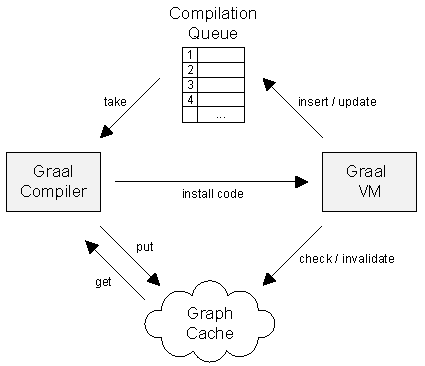
\includegraphics[width=0.75\textwidth]{graal_architecture.pdf}
\end{table}
\end{frame}

\begin{explainframe}{Graal VM - Details}
\begin{enumerate}
    \item Graal VM detects \textit{hot} methods
    \item Graal VM adds these methods to compilation queue
    \item Compiler threads compile methods with highest priorities
    \item Machine code is installed into runtime's cache
\end{enumerate}
\end{explainframe}

\begin{frame}{JRuby, Truffle and Graal: Overview of Threads}
\begin{table}
    \centering
    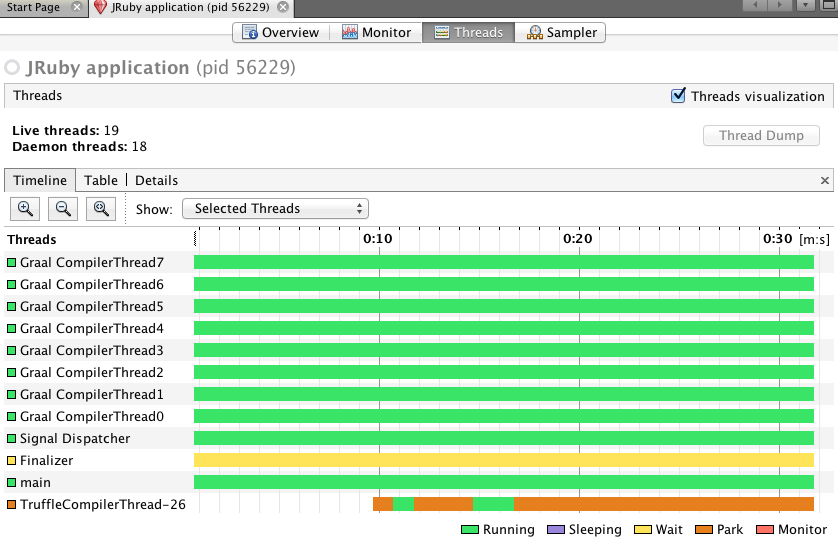
\includegraphics[width=1.0\textwidth]{visualvm.png}
\end{table}
\end{frame}

\section{Truffle in Practice}

\begin{frame}{Ways to use Truffle within an existing AST Interpreter}

\begin{description}
 \item[Convert to Truffle:] Translate all AST nodes to Truffle nodes
 \item[Add-On Truffle:] Add an additional set of AST nodes
\end{description}
\begin{table}
  \centering
  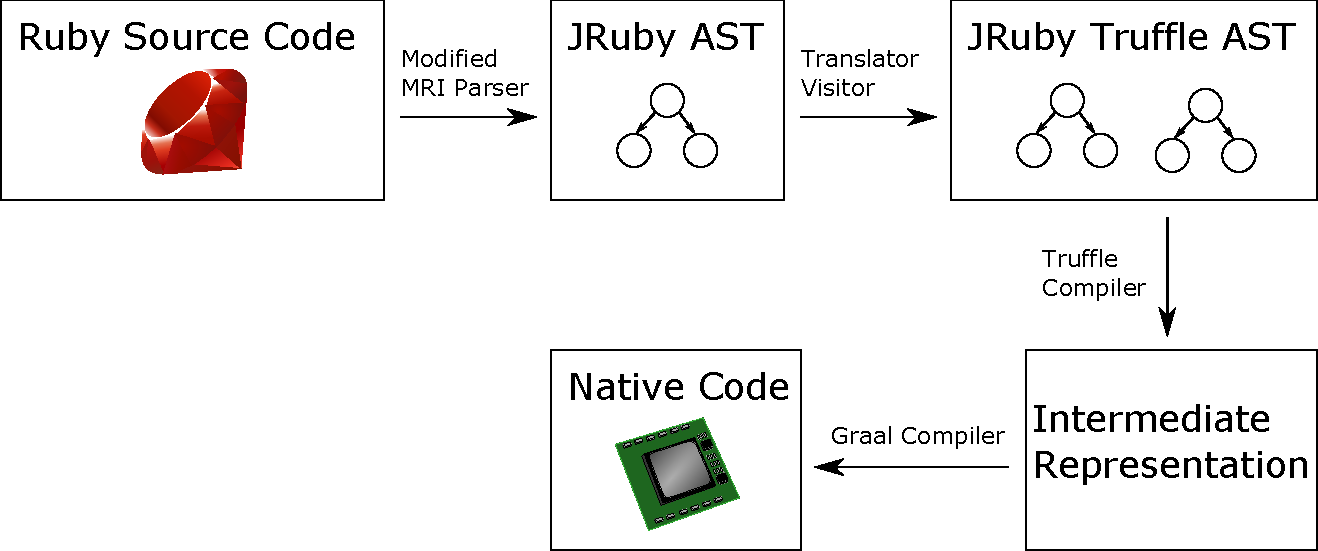
\includegraphics[width=1.0\textwidth]{graaltruffle.pdf}
\end{table}
\end{frame}

\begin{frame}{Method Call Nodes in (J)Ruby}
\begin{table}
    \centering
    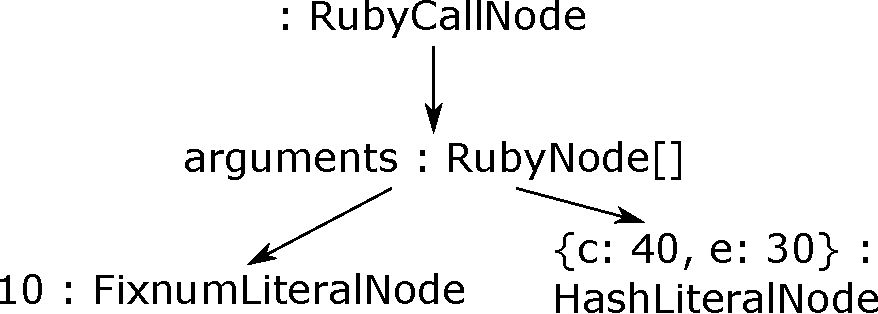
\includegraphics[width=0.75\textwidth]{kwarg_1.pdf}
\end{table}

\begin{itemize}
    \item \lstinline{RubyCallNode} contains:
      \begin{itemize}
      \item Receiver object
      \item Method name (fix)
      \item List of argument AST nodes
      \item Block AST node
      \end{itemize}
    \item Dynamic call $\rightarrow$ Dynamic dispatch is run on every execution
\end{itemize}
\end{frame}

\begin{frame}{Method Callee Node in (J)Ruby}
\begin{enumerate}
 \item \lstinline{RubyRootNode}
 \item \lstinline{Catch*Nodes} (\lstinline{CatchNextNode}, \lstinline{CatchRetryAsErrorNode}, \lstinline{CatchReturnNode} \dots)
 \item \lstinline{SequenceNode} \begin{enumerate}
    \item \lstinline{CheckArityNode}
    \item \lstinline{WriteLocalVariableNode} for argument 1
    \item \lstinline{WriteLocalVariableNode} for argument 2
    \item \lstinline{WriteLocalVariableNode} for kwargument e
    \item \lstinline{WriteLocalVariableNode} for kwargument c
    \item Statement sequence itself (wrapped in \lstinline{TracingNodes}, with \lstinline{CyclicAssumption}s)
  \end{enumerate}
\end{enumerate}
Nice: Every argument has a node to create its default argument, maybe a node that throws every time a exception
\end{frame}



\section{Challenge: Optimize Keyword Arguments in JRuby}

\begin{frame}[fragile]{Task: Keyword Arguments in Ruby 2.x}

\begin{itemize}
 \item Shortcut to call method with dictionary as last argument:
    \begin{lstlisting}
    method(10, e: 30, c: 40)
    method(10, {:e => 30, :c => 40})
    \end{lstlisting}
  \item Starting with Ruby 2.0, Ruby can process this dictionary automatically (so called keyword arguments):
    \begin{lstlisting}
    def method(a, b=3, e:, c:30)
    end
    \end{lstlisting}
\end{itemize}
\end{frame}

%\begin{frame}{First Optimizations}
%\begin{itemize}
% \item Reduce duplicate method calls
% \item Using iterators to improve RubyHash handling
%\end{itemize}
%\end{frame}

\subsection{Problem}

\begin{frame}{Performance Bottlenecks}
\begin{itemize}
    \item \lstinline{Hash} object creation: object is created, passed as argument, then destructed again
    \item Inefficient code paths (e.g., multiple scans of \lstinline{Hash} object)
    \item Code involving \lstinline{Hash} objects is harder to optimize than code involving primitive objects (Graal optimizations)
    \item Keyword argument nodes are not optimized by Truffle (Java \lstinline{equals}, Truffle boundary for \lstinline{Hash} iterator)
    \item Execution remains in interpreter modus
\end{itemize}

\begin{table}
    \centering
\textbf{Goal: Pass keyword arguments as normal arguments}
\end{table}
\end{frame}


\subsection{Solution}
\begin{frame}{Optimizations}
\begin{enumerate}
 \item Optimize implementations (efficient hash operations)
 \item Store kwargs within normal arguments array, separated by marker
 \item Cache kwargs mapping within dispatch chain
\end{enumerate}

$\rightarrow$ We will now look into optimization \#3
\end{frame}

\begin{explainframe}{Fully Optimized Keyword Arguments}{Callee's Point of View}
\begin{itemize}
    \item \lstinline{VirtualFrame} contains \lstinline{arguments} array.
    \item Array contains \lstinline{Marker} object, generated by \lstinline{MarkerNode} as last element, if call is optimized.
    \item \lstinline{CachedBoxedDispatchNode} is always optimized if keyword arguments are present (rewriting of \lstinline{argumentNodes} array).
    \item \lstinline{ReadKeywordArgumentNode} has offset (from right side) into \lstinline{arguments} array as instance variable.
    \item \lstinline{ReadKeywordArgumentNode} accesses \lstinline{arguments} array at offset if call is optimized, otherwise expects a \lstinline{RubyHash} (old behavior).
    \item \lstinline{CachedBoxedDispatchNode} might generate an additional \lstinline{RubyHash} if rest keyword arguments are present.
\end{itemize}
\end{explainframe}

\begin{frame}[fragile]{Fully Optimized Keyword Arguments}{Example}
\begin{lstlisting}
class Cls1
    def method(a:, **kwargs)
    end
end

class Cls2
    def method(a:, b:)
    end
end

[Cls1.new, Cls2.new].each do |obj|
   obj.method(a: 1, b: 2)
end
\end{lstlisting}
\end{frame}

\begin{frame}{Recap: Type Decision Chains}{Source: ``Self-Optimizing AST Interpreters''}
\begin{table}
    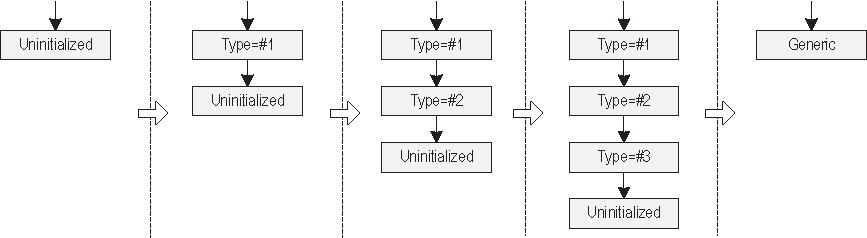
\includegraphics[width=\textwidth]{type_chain.pdf}
\end{table}
\end{frame}

\begin{frame}{Fully Optimized Keyword Arguments}{Problems}
\begin{itemize}
    \item Nodes are specific with regard to user-defined Ruby classes \\ (cannot use Truffle DSL)
    \item Truffle DSL supports only specialization for language types
    \item Type of receiver is not known before dispatching the call
\end{itemize}
\end{frame}

\begin{frame}{Guest Language PIC in JRuby}
\begin{table}
    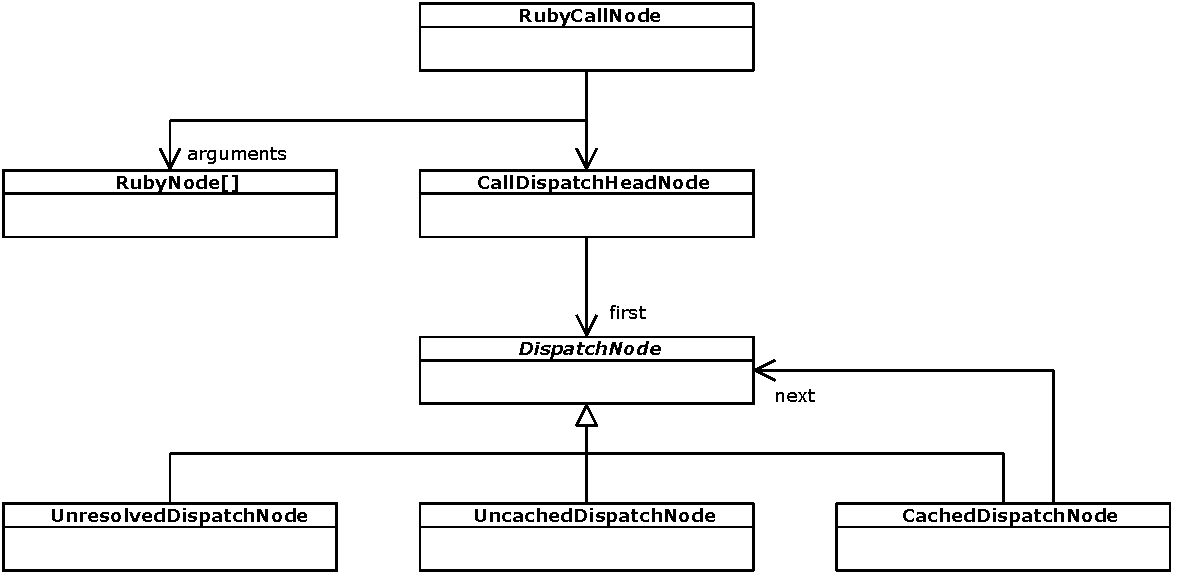
\includegraphics[width=\textwidth]{dispatch.pdf}
\end{table}
\end{frame}

\begin{explainframe}{Guest Language PIC in JRuby}
\begin{itemize}
    \item \lstinline{UnresolvedDispatchNode}: corresponds to Truffle's \emph{unspecified node}
    \item \lstinline{UncachedDispatchNode}: corresponds to Truffle's \emph{generic node}
    \item \lstinline{CachedDispatchNode}: corresponds to Truffle's \emph{specialized nodes}
    \item Node rewriting similar to Truffle but without Truffle
\end{itemize}
\end{explainframe}

\begin{frame}{Argument Passing in \textit{DispatchNode}}
\begin{table}
    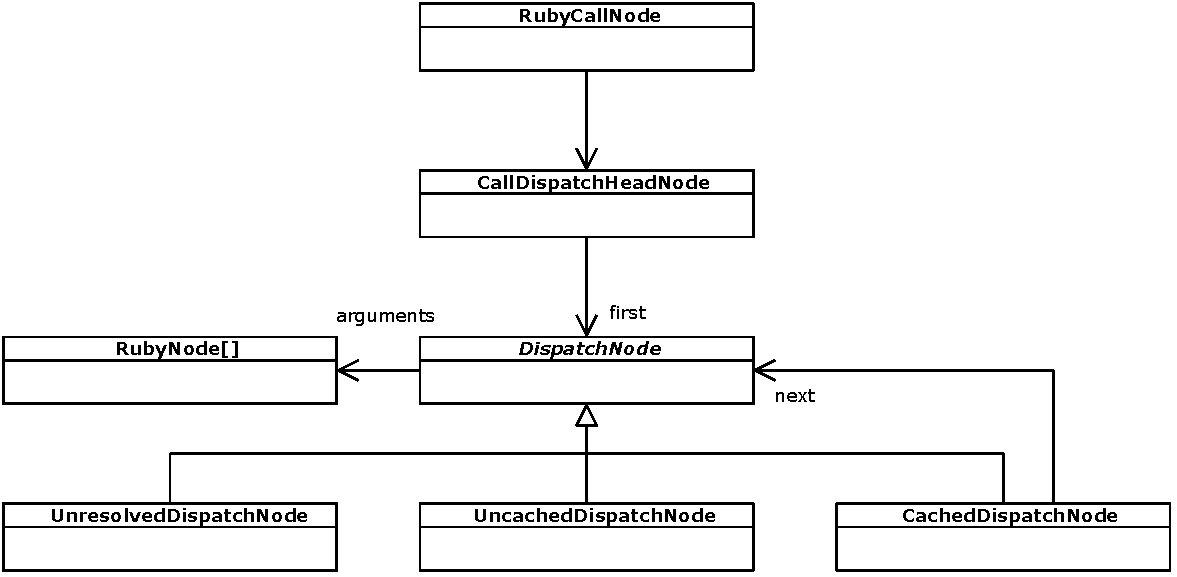
\includegraphics[width=\textwidth]{dispatch_opt.pdf}
\end{table}
\end{frame}

\begin{explainframe}{Argument Passing in \lstinline{DispatchNode}}
\begin{itemize}
    \item Unmodified arguments array (possible with \lstinline{HashLiteralNode}) is stored in \lstinline{UnresolvedDispatchNode}
    \item \lstinline{CachedDispatchNode} contains keyword arguments mentioned in signature in array, and other keyword arguments in \lstinline{HashLiteralNode}
    \item \lstinline{ReadKeywordArgumentNode} checks if method dispatch is optimized (marker present in arguments array) and reads keyword arguments from arguments array, otherwise extracts them from \lstinline{Hash} (same as before)
\end{itemize}
\end{explainframe}

\begin{frame}{Evaluation}
\begin{exampleblock}{Results}
Keyword arguments are as fast as position arguments

(for specific but common cases)
\end{exampleblock}
\end{frame}


\begin{explainframe}{Evaluation}

$\rightarrow$ Keyword arguments are as fast as position arguments
\begin{itemize}
    \item Optimization affects only arguments passed in keyword argument syntax in method calls
    \item Optimization does not affect keyword arguments passed as an already existing \lstinline{Hash}
\end{itemize}
\end{explainframe}


\section{Summary}
%%%%%%%%%%%%%%%%%

\begin{frame}{Truffle Summary}
\begin{itemize}
 \item Specific Java code cannot be translated by Graal (or it is disallowed)
 \item Large AST interpreters can still get unclear/distracting, knowledge is the composition of nodes, not the nodes itself
 \item Truffle DSL is not enough for efficient implementation of complex languages
 \item It is still needed to write efficient code and node implementations
\end{itemize}
\end{frame}

\begin{frame}{Truffle and RPython - A Very Subjective Comparison}
\begin{description}
 \item[RPython] \begin{itemize}
  \item Lightweight stack
  \item A little bit easier to get to work - mostly getting the correct libs in the Python path
  \item Difficult to debug in depth what is happening at execution
\end{itemize}
\item[Truffle] \begin{itemize}
  \item Heavy stack (Java, mostly multiple JDK and often maven \dots)
  \item If you get it working, you have the full power of (debugging) Java, even Graal itself
\end{itemize}
\end{description}
\end{frame}


\section{References}
%%%%%%%%%%%%%%%%%

\begin{frame}{References}
\begin{itemize}
 \item L. Stadler, G. Duboscq, H. Mössenböck, T. Wurthinger, \textbf{Compilation Queuing and Graph Caching for Dynamic Compilers}, \small{\url{http://lafo.ssw.uni-linz.ac.at/papers/2012_VMIL_Graal.pdf}}
 \item T. Würthinger, C. Wimmer, A. Wöß, L. Stadler, G. Duboscq, C. Humer, G. Richards, D. Simon, M. Wolczko. \textbf{One VM to Rule Them All}, 2013, \small{\url{http://lafo.ssw.uni-linz.ac.at/papers/2013_Onward_OneVMToRuleThemAll.pdf}}
 \item T. Würthinger, A. Woß, L. Stadler, G. Duboscq, D. Simon, C. Wimmer. \textbf{Self-Optimizing AST Interpreters}, 2012, \small{\url{http://lafo.ssw.uni-linz.ac.at/papers/2012_DLS_SelfOptimizingASTInterpreters.pdf}}
 \item Graal (\url{http://hg.openjdk.java.net/graal/graal})
 \item JRuby (\url{https://github.com/jruby/jruby})
 \item JRuby Developers (especially Chris Seaton)
 \item JRuby Benchmarks (\url{https://github.com/jruby/bench9000})
\end{itemize}
\end{frame}

\end{document}
